
\documentclass{beamer}

%\setbeameroption{show notes on second screen=right} % Make sure slide position is set to "right" in pympress also, or if using pdfpc, with --notes=right
% Also, comment out the notes to produce slides for archiving, etc.
\usetheme{Berlin}
%Note: use pympress on the rendered pdf to have things like second screen, notes, etc! Cool!

%title page details:
\title{\LaTeX{} Engineering Grad Society Presentation}
\subtitle{A presentation about \LaTeX{} to the McMaster EGS}
\author{John Fink}
\institute{McMaster University}
\date{July 19th, 2022}


\begin{document}

	\begin{frame}
		\titlepage
	\end{frame}

	\begin{frame}
		Who am I?
	\end{frame}

\begin{frame}
	What is the difference between \textit{word processing} and \textit{typesetting}?
\end{frame}

\begin{frame}
	Why choose typesetting over (most) word processing?
	\begin{itemize}
		\item Item 1
		\pause
		\item Item 2
		\pause
		\item Item 3  
	\end{itemize}
\end{frame}

\begin{frame}
	\begin{itemize}
		\item Worry about \textbf{content}, not (or not much) about \textbf{form}.
	\end{itemize}
\end{frame}

\begin{frame}
	\begin{itemize}
		\item Long term preservation	
	\end{itemize} 
	\note{Bloomsday book example? Agrippa? Or just talk about how it is about 100000x easier to do programmy-type things -- like git version control etc -- on plain text vs. some sort of weird homunculus like word}
\end{frame}

\begin{frame}
	%insert word doing dumb thing here
\end{frame}

\begin{frame}
	Why choose word processing \textit{over} typesetting?
	\note{this is a note.}
\end{frame}

\begin{frame}
	What is \LaTeX{}?
\end{frame}

\begin{frame}
	What is... TeX?
	\note{wikpedia sez: "is a typesetting system which was designed and written by Donald Knuth[1] and first released in 1978. TeX is a popular means of typesetting complex mathematical formulae; it has been noted as one of the most sophisticated digital typographical systems."}
\end{frame}

\begin{frame}
	The \textbf{structure} of a \LaTeX{} document.
	\note{a LaTeX document is *just text*. You can edit it with anything that edits plain text and doesn't mangle it, you can put it in version control, you can copy it anywhere, you can be assured that -- as plain text -- it will probably be viewable, at least as text, for the forseeable future (my lifetime, if not yours at least)}
\end{frame}

\begin{frame}
	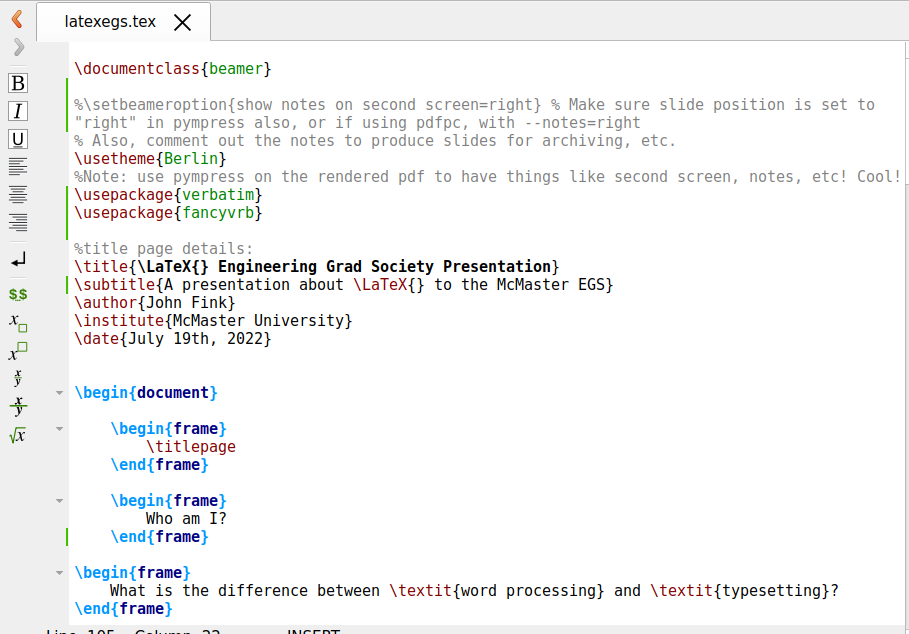
\includegraphics[height=8cm]{latex-structure}
\end{frame}

\begin{frame}
	%this is always the last slide
	Any questions?
\end{frame}
	
\end{document}